\section{Data Driven Application}

\fixme{List effects in data}

\subsection{Fit of the Dijet Asymmetry}

The dijet pdf~\qeq{eq:ResFit:DijetPdf} is in fact equivalent to a pdf of the dijet
asymmetry with an additional assumption for the underlying particle
level jet spectrum, as will be shown in this section.

The dijet asymmetry is defined as
\begin{equation}\label{eq:ResFit:Asymmetry}
  A = \frac{\pti{1'}-\pti{2'}}{\pti{1'}+\pti{2'}},
\end{equation}
where \pti{1'} and \pti{2'} refer to the randomly ordered transverse momenta of the
leading two jets in an event.
In case of events with exactly two jets of same particle level jet
transverse momentum \pt and Gaussian response, the width $\sigma(A)$ of the asymmetry distribution is
related to the jet \pt resolution $\sigma$ by
\begin{equation*}
  \sigma(A) = \frac{1}{\sqrt{2}}\frac{\sigma}{\pt}.
\end{equation*}

Additional acitivity in the events, e.g. from soft gluon radiation, as
well as out-of-cone effects during the jet clustering bias the dijet asymmery and have to be
corrected for when measuring the resolution.
That is discussed in detail in \qsec {sec:ResFit:AddJets}; the rest of
this section is devoted to the comparison of the performance of a
binned and an unbinned fit of the dijet asymmetry.
The completely analogue case is demonstrated in
\qsec{sec:ResFit:Asym:SimpleFit} where the likelihood is simplified by replacing the spectrum
with the assumption \mbox{$\pttrue = \ptave$}.
Since the unbinned fit is more sensitive to non-Gaussian tails, an outlier
suppression technique is introduced.
In \qsec{sec:ResFit:Asym:FullFit}, the full dijet pdf, including an assumption for the
spectrum, is finally used to fit the asymmetry;
the spectrum is also used to derive a better estimator for \ptgen.


\subsubsection{Simple Maximum Likelihood Fit and Outlier Treatment}\label{sec:ResFit:Asym:SimpleFit}

If the spectrum $f$ in the dijet pdf~\qeq{eq:ResFit:DijetPdfTransformed} is replaced by \mbox{$f(\pttrue)  = \delta\left(\pttrue - \ptave\right)$}, i.e. the assumption \mbox{$\pttrue = \ptave$}, 
\qeq{eq:ResFit:DijetPdfTransformed} simplifies to
\begin{equation}
\label{eq:ResFit::DijetPdfTransformed:Simple}
  g_{\sigma'}\left(\Delta\pt\right) \propto
  \e^{-\frac{1}{2}\left(\frac{\Delta\pt}{\sigma'}\right)^{2}}, 
\end{equation}
with \mbox{$\sigma' = \sigma/\sqrt{2}$}.
This corresponds to the pdf of the asymmetry in the event, assuming
Gaussian response.

In real data, however, there are non-Gaussian tails biasing the fit of the asymmetry.
In case of a binned fit of the histogram, the influence of the tails is suppressed by
fitting only the bulk of the distribution, defined as two standard deviations around the mean.
In case of the unbinned fit, it is not as straight
forward to select only the bulk events.
This can be achieved, however, with an iterative procedure by restricting
the allowed range of $\Delta\pt$.
As observed in data and MC simulation (\fixme{reference to plot}), tails start to appear for \mbox{$|\Delta\pt| > 2\sigma'$}.
Hence, the unbinned fit is performed only for events with \mbox{$|\Delta\pt| < 2\sigma'$}.
In order to preserve unitarity of the dijet pdf, the normailisation
of~\qeq{eq:ResFit::DijetPdfTransformed:Simple} is adapted accordingly.
\fixme{State complete pdf in Appendix}

The threshold on $|\Delta\pt|$ in the above choice is proportional to $\sigma'$, which is the fitted parameter, and would be varied accordingly during the maximisation.
This, however, biases the result towards smaller \fixme{???} values.
Therefore the threshold is kept fixed and the maximisation is iterated
four times, leading to an unbiased result.

\begin{figure}[ht]
  \label{fig:ResFit:Asym:Simple}
  \centering
  \begin{tabular}{cc}
    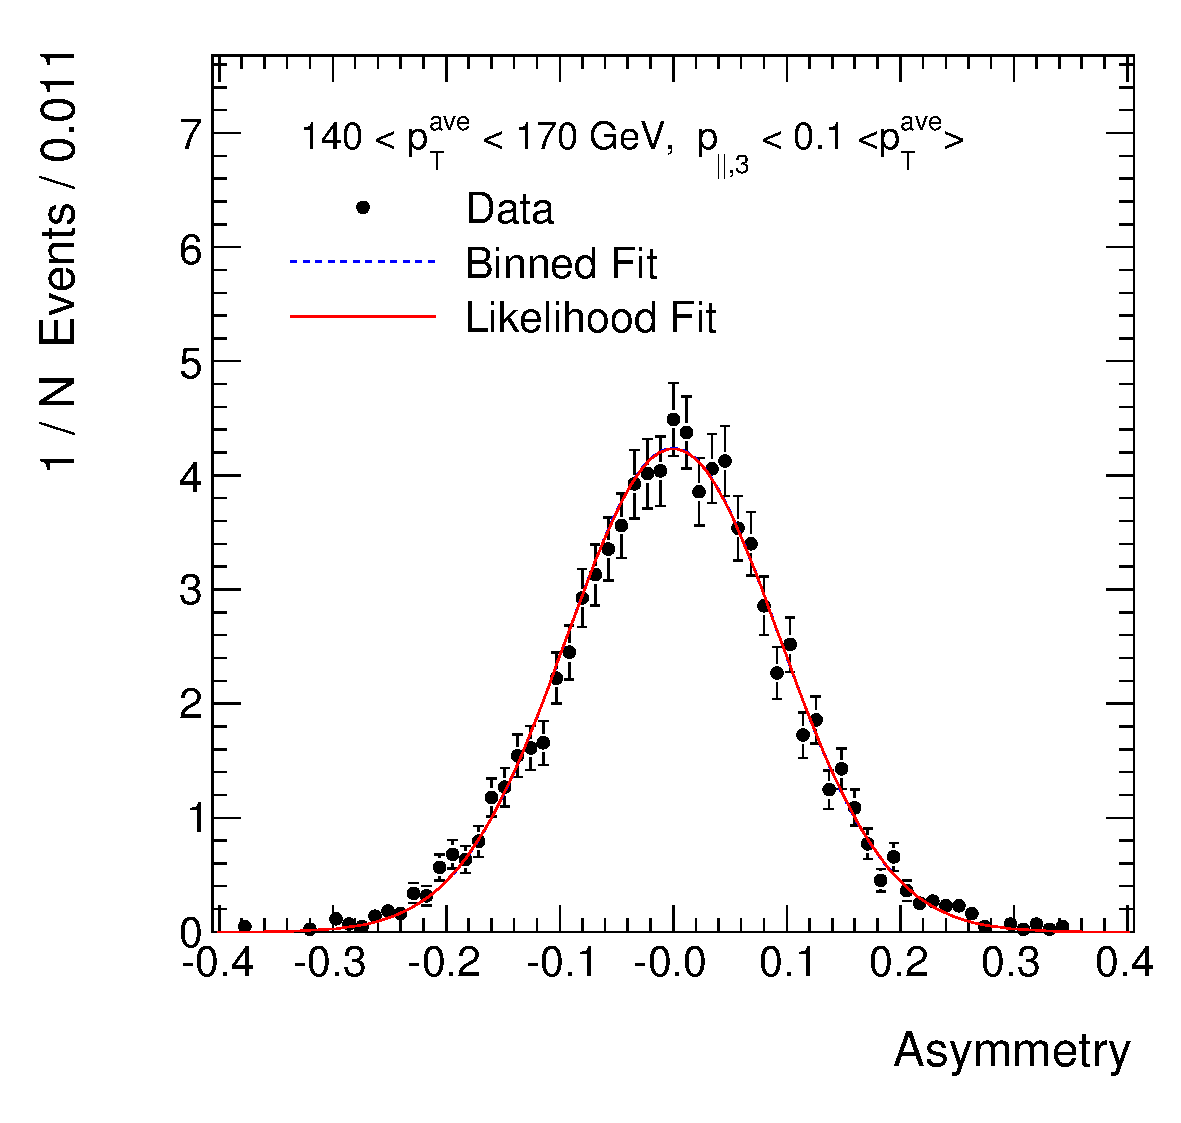
\includegraphics[width=0.45\textwidth]{figures/MaxLikeSimple_Data132440-144011_Eta00-13_PtAsymmetry_PtBin4_Pt3Cut3} &
    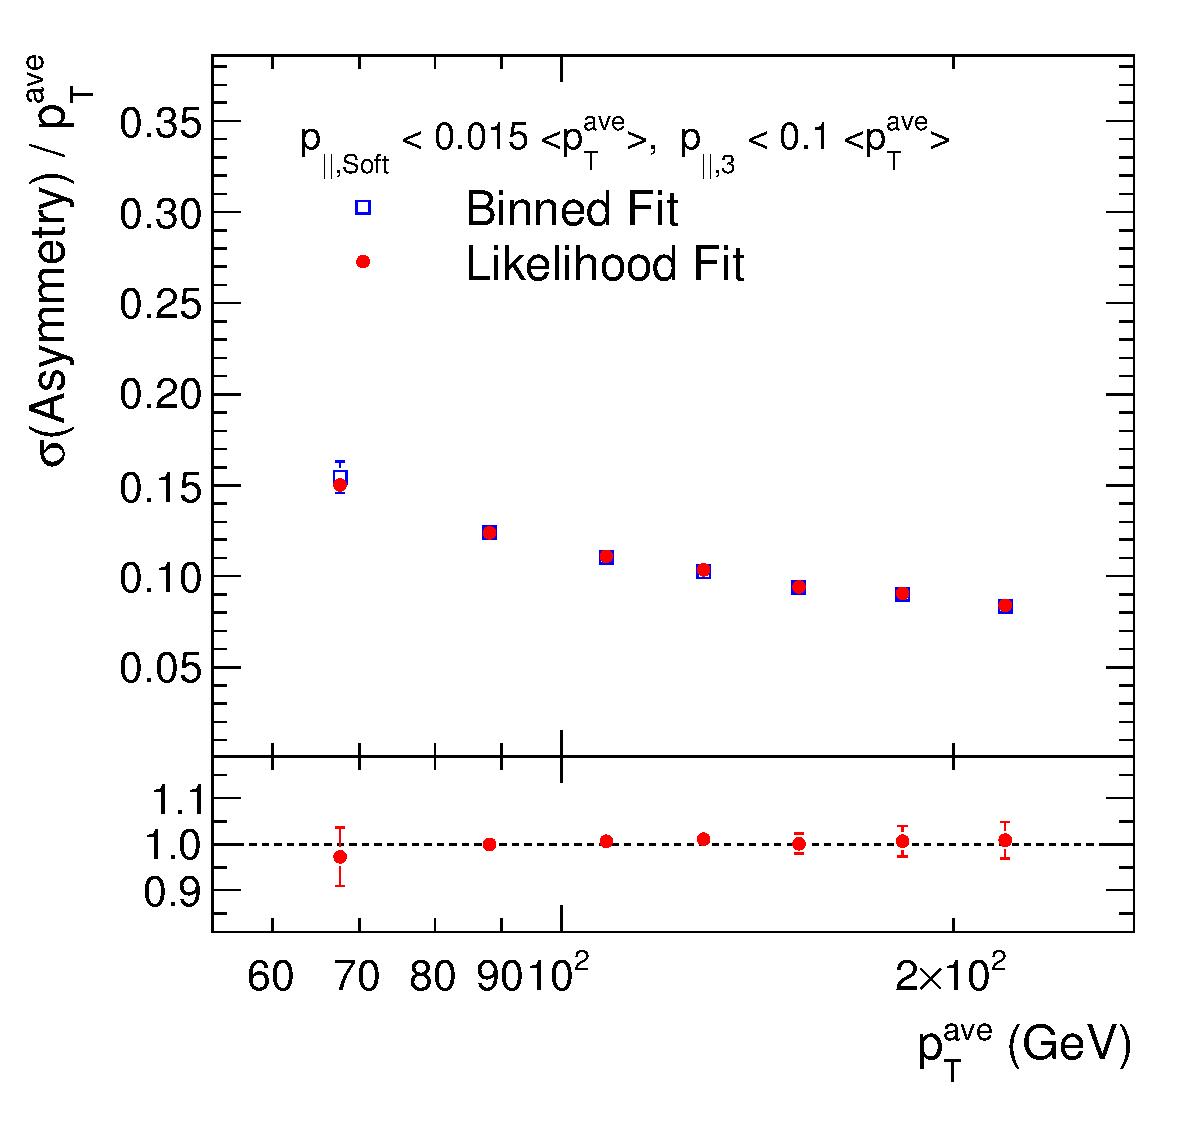
\includegraphics[width=0.45\textwidth]{figures/MaxLikeSimple_Data132440-144011_Eta00-13_PtAsymmetryWidthBottomRatio_Pt3Cut3} \\
\end{tabular}
  \caption{(\textit{Left}) Dijet asymmetry distribution measured in
    Collider data (circles) for \mbox{$\ppi{3} < 0.1\cdot\mean{\ptave}$} and \mbox{$\ppi{\text{Soft}} < 0.015\cdot\mean{\ptave}$} in the \mbox{$140 < \ptave < 170\gev$} bin.
    It is well described by the prediction (solid line) from the
    simplified unbinned maximum likelihood fit and there is good agreement to a direct binned
    fit (dashed line) of the histogram.
    Note that both lines lie in fact on top of each other.
    (\textit{Right}) Width of the asymmetry distributions from
    Collider data in different \ptave bins from binned Gaussian fits to the
    histograms (open squares) in comparison to the predictions from
    the unbinned fit (solid circles).}
\end{figure}

The asymmetry distribution measured in Collider data for \mbox{$140 < \ptave < 170\gev$}, \mbox{$\ppi{3} < 0.1\cdot\mean{\ptave}$}, and \mbox{$\ppi{\text{Soft}} < 0.015\cdot\mean{\ptave}$} is shown in \qsubfig{fig:ResFit:Asym:Simple}{left}.
It is well described by the result of the discussed simplified unbinned fit, i.e. a Gaussian with width $\sigma'$, and there is good agreement to a direct binned fit of the histogram.
In \qsubfig{fig:ResFit:Asym:Simple}{right}, the widths $\sigma'$ measured in different \ptave bins with the unbinned technique are further compared to the results of binned fits.
Again, there is good agreement.

In conclusion, the simplified unbinned likelihood fit of the asymmetry performs equally to a binned fit of corresponding histogram.



\subsubsection{Full Maximum Likelihood Fit Including the Spectrum and Description of the Selection Bias}\label{sec:ResFit:Asym:FullFit}

In the following, the extension of the dijet pdf with an assumption for the particle level jet \pt cross section $f$ is discussed.
With the choice of coordinates~\qeq{eq:ResFit:TransformedCoordinates}, this corresponds to multiplying a pdf for the measured \ptave,
\begin{equation*}
\label{eq:ResFit::DijetPdfTransformed:Simple}
  g_{\sigma'}\left(\ptave\right) \propto
  \int\dif{\pttrue}\;f\left(\pttrue\right)\cdot
  \e^{-\frac{1}{2}\left(\frac{\ptave - \pttrue}{\sigma'}\right)^{2}} \, , 
\end{equation*}
resulting in~\qeq{eq:ResFit:DijetPdfTransformed}.
As mentioned before, the spectrum is taken from the MC simulation (\qsubfig{fig:ResFit:Asym:Spectrum}{left}) and not modified during the fit.
The resulting systematic uncertatinties have to be evaluated.

By this extension, additionally a description of biases in the event selection can be included into the likelihood.
Binning in (measured) \ptave causes migration effects at the edges of the selected \ptave range due to the finite jet \pt resolution:
there are jets that fluctuate either into or out of the selected interval.
This is illustrated in \qsubfig{fig:ResFit:Asym:Spectrum}{right} with simulated data using the MC truth information.
Additionally, because of the steeply falling dijet \pt spectrum, there are more jets that fluctuate high than jets that fluctuate low in \pt and the selected sample is therefore biased towards jets of lower \ptgen that fluctuated high in the detector.

\begin{figure}[ht]
  \label{fig:ResFit:Asym:Spectrum}
  \centering
  \begin{tabular}{cc}
    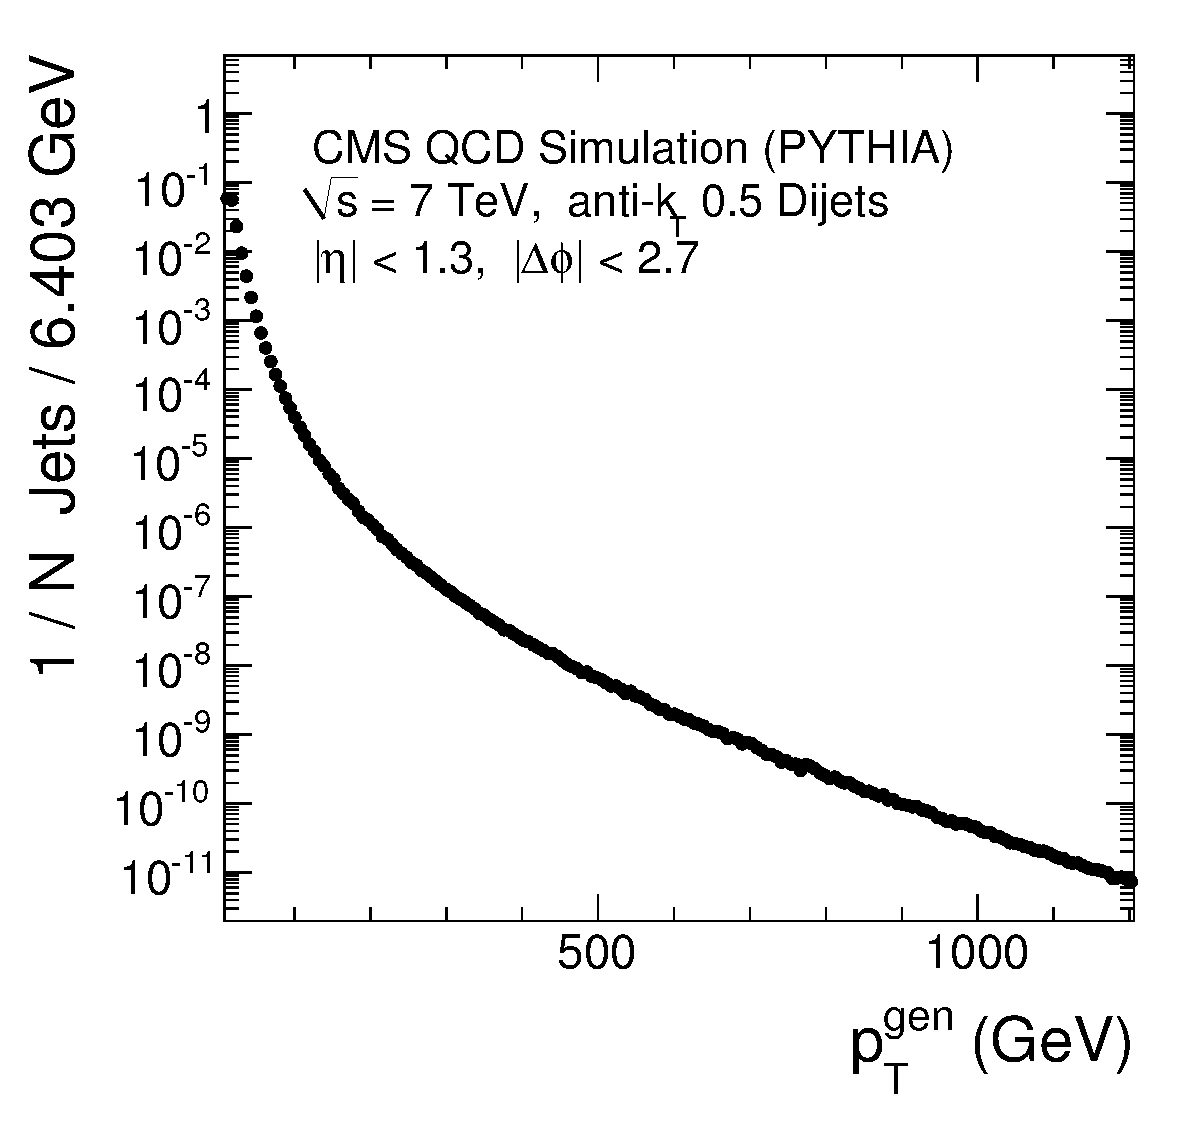
\includegraphics[width=0.45\textwidth]{figures/ExampleSpectrum} &
    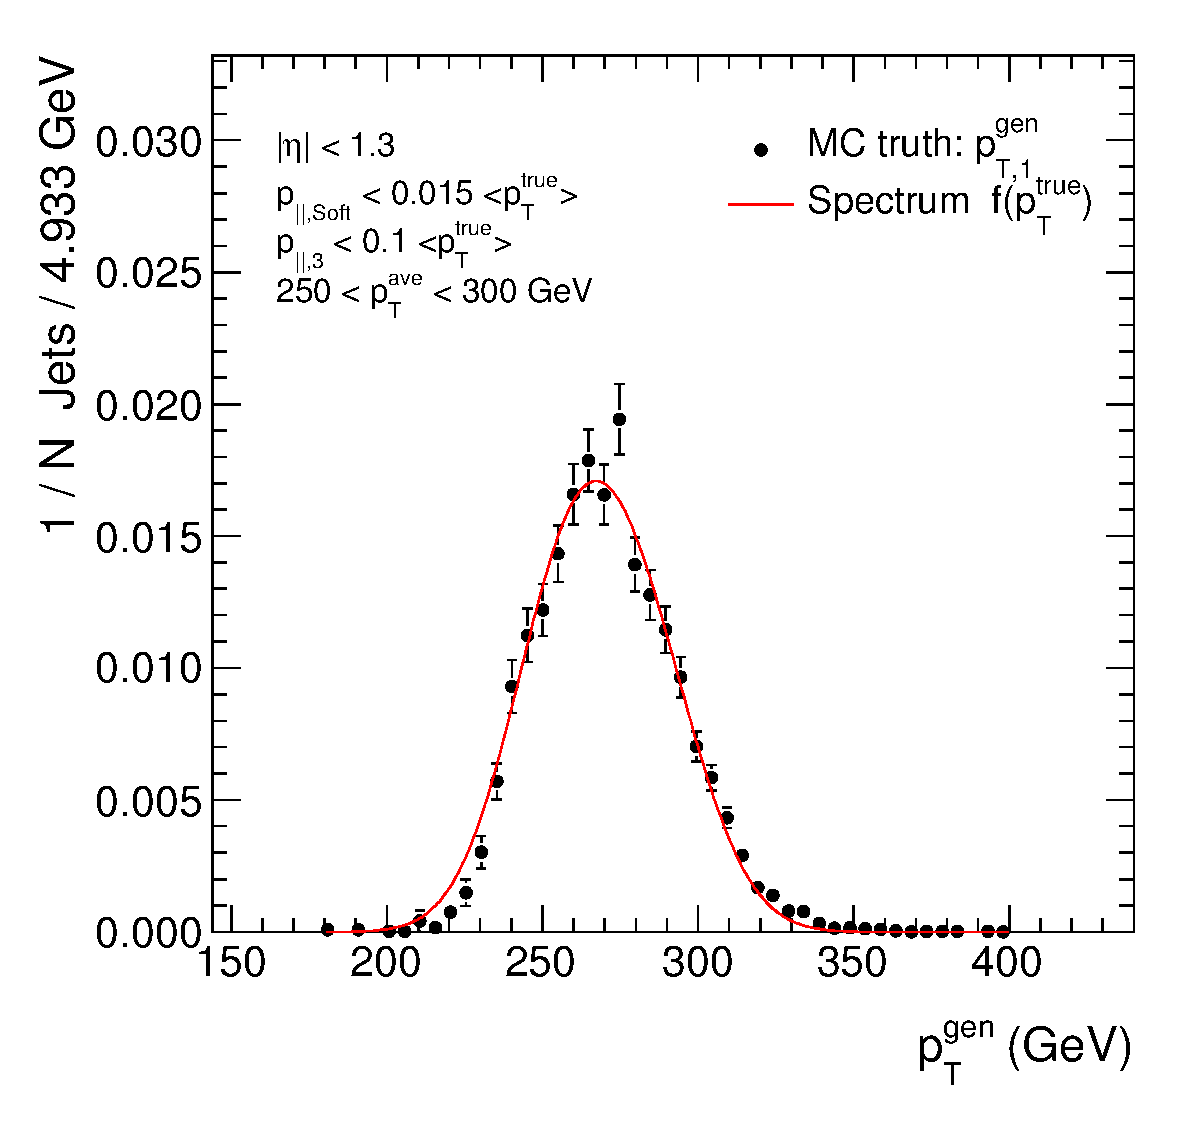
\includegraphics[width=0.45\textwidth]{figures/MaxLike_Eta00-13_SpectrumJet1_PtBin7}\\
 \end{tabular}
  \caption{(\textit{Left}) Dijet \ptgen spectrum from the MC simulation.
    Per selected event, the \ptgen of both the leading jets has been filled into the histogram.
    A linear interpolation of this histogram is used as the particle level differential jet cross section in~\qeq{eq:ResFit:Asym:ModifiedSpectrum}.
    (\textit{Right}) \ptgen spectrum (circles) of the selected dijet events in the \mbox{$250 < \ptave < 300\gev$} bin.
    It is well described by the modified cross section $f$ in~\qeq{eq:ResFit:Asym:ModifiedSpectrum} (solid line).}
\end{figure}

The dijet pdf~\qeq{eq:ResFit:DijetPdfTransformed} is modified to describe the
\ptave selection and hence avoid biasing the measured resolution.
First, the allowed range of \ptave is considered in the normalisation. \fixme{Reference to Appendix}
Second, the \pttrue pdf is extended to incorporate the migration effects:
\begin{equation}
  \label{eq:ResFit:Asym:ModifiedSpectrum}
  f\left(\pttrue\right) = \frac{1}{\mathcal{N}_{f}}
  f_{0}\left(\pttrue\right) \int^{\ptavemax}_{\ptavemin}\dif{x}\;\mathcal{G}\left(x|\sigma',\pttrue\right) \, ,
\end{equation}
Here, $f_{0}$ denotes the underlying particle level jet \pt spectrum \qsubfig{fig:ResFit:Asym:Spectrum}{left}\footnote{The actual probability densities are evaluated using a linear interpolation of the histogram.} and $\mathcal{G}$ is a Gaussian of width \mbox{$\sigma' = \sigma/\sqrt{2}$}, i.e. the pdf of \ptave for a given \pttrue.
Equation~\qeq{eq:ResFit:Asym:ModifiedSpectrum} is validated using simulate data:
the \ptgen spectrum of selected dijet events is well described by $f(\pttrue)$ as demonstrated in \qsubfig{fig:ResFit:Asym:Spectrum}{right}.
This extension to $f$ depends solely on the fitted parameter $\sigma'$ and does not introduce any new dependencies on the MC simulation.





\subsection{Influence of Additional Hadronic Activity and Hadronisation Effects}\label{sec:ResFit:AddJets}


\subsubsection{Contributions to the Dijet Asymmetry}\label{sec:ResFit:AddJets:Contributions}

The dijet probability density function
in~\eqref{eq:qcd:resolMaxlike:dijetPdf} is constructed under the
assumption of \pt balance at particle jet level.
Any additional jet with a component of \pt along the dijet
axis\footnote{The dijet axis $\phi_{||}$ is defined as the direction normal to the
angle bisector of the leading two jets.} causes an
imbalance which biases the measured resolution, as
illustrated in Fig.~\ref{fig:qcd:resolMaxlike:biasAddJets}.

\begin{figure}[ht]
  \centering
  \begin{tabular}{cc}
    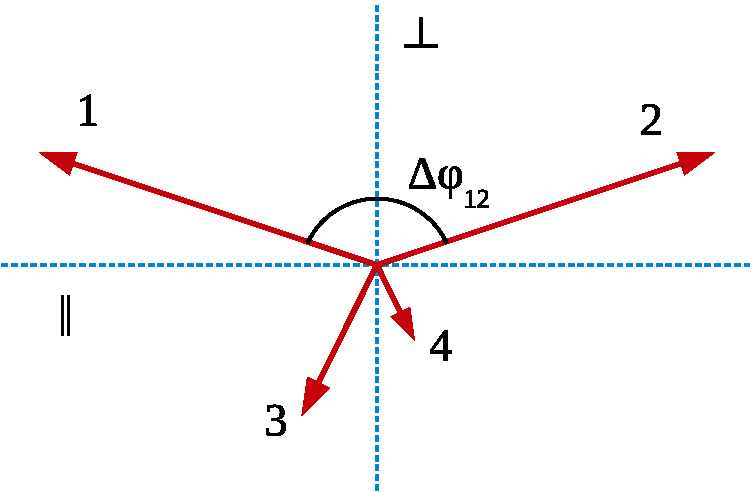
\includegraphics[width=0.45\textwidth]{figures/Sketch_Projections}
    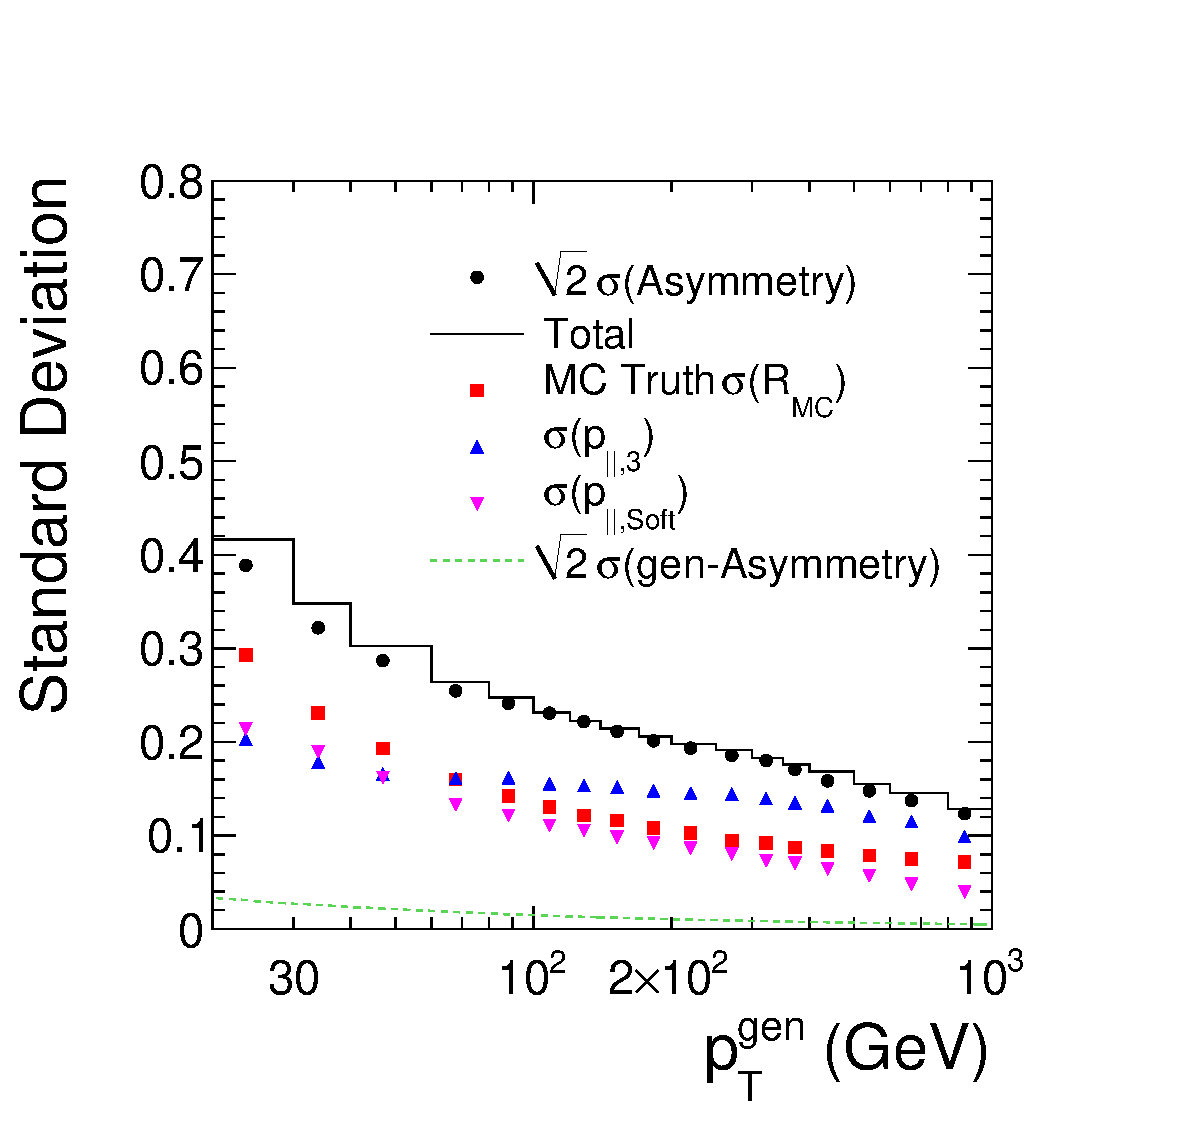
\includegraphics[width=0.45\textwidth]{figures/Spring10QCDDiJet_ParallelComponent_hParallelContributions}\\
  \end{tabular}
  \caption{(\textit{Left}) Definition of the dijet axis $\phi_{||}$, the direction normal to the
    angle bisector of the leading two jets in the transverse plane.
    Additional jets with \pt components along $\phi_{||}$ will cause
    a \pt imbalance of the particle jets and bias the measured
    resolution towards larger values.
    (\textit{Right}) Gaussian resolutions \mbox{$\sigma/\mean{\pttrue}$} measured with the unbinned
    fit in Collider data for \mbox{$140 < \ptave < 170\gev$} and different \ppi{3}
    thresholds after suppression of additional soft jet activity along
    $\phi_{||}$. 
    \mbox{$\sigma/\mean{\pttrue}$} on \ppi{3} is linearly
    extrapolated to the case of an ideal dijet event.
  }
  \label{fig:qcd:resolMaxlike:biasAddJets}
\end{figure}


\subsubsection{Correction for Additional Hadronic Activity}\label{sec:ResFit:AddJets:Extrapolation}



\fixme{Motivate binned approach}

In order to compensate for the influence of additional jet activity,
events are selected in reasonably small bins of \ptave.
Per bin, the \pt components along the dijet axis $\phi_{||}$ of the third and all further jets,
\begin{eqnarray*}
  \ppi{3} & = & |\pti{3}\cos(\phi_{3}-\phi_{||})| \\
  \ppi{\text{Soft}} & = & |\sum_{i>3}\pti{i}\cos(\phi_{i}-\phi_{||})|,
\end{eqnarray*}
are restricted to
\begin{eqnarray*}
  \ppi{3} & < & z\cdot\mean{\pttrue} \\
  \ppi{\text{Soft}} & < & 0.015\cdot\mean{\pttrue},
\end{eqnarray*}
where $\mean{\pttrue}$ is the mean particle level jet \pt in that bin
as computed from the assumed spectrum $f(\pttrue)$
in~\eqref{eq:qcd:resolMaxlike:toyMC:ptCuts:extendedSpectrum}.
Several sets of dijet events are selected, each with a different
threshold $z$ of \ppi{3}, and the mean Gaussian response with \pt
independent resolution $\sigma$ is fitted by maximising the dijet
likelihood~\eqref{eq:qcd:resolMaxlike:likelihood} w.r.t. $\sigma$.
The dependence of the jet \pt resolution on the $z$ is clearly visible in Fig.~\ref{fig:qcd:resolMaxlike:biasAddJets}.
In order to extrapolate the measurement to the case of a two jet only
event, the \mbox{$\sigma/\mean{\pttrue}$} are fitted with a linear
function and the $y$ axis intercept is taken as the unbiased jet \pt
resolution.

\begin{figure}[ht]
  \centering
  \begin{tabular}{cc}
    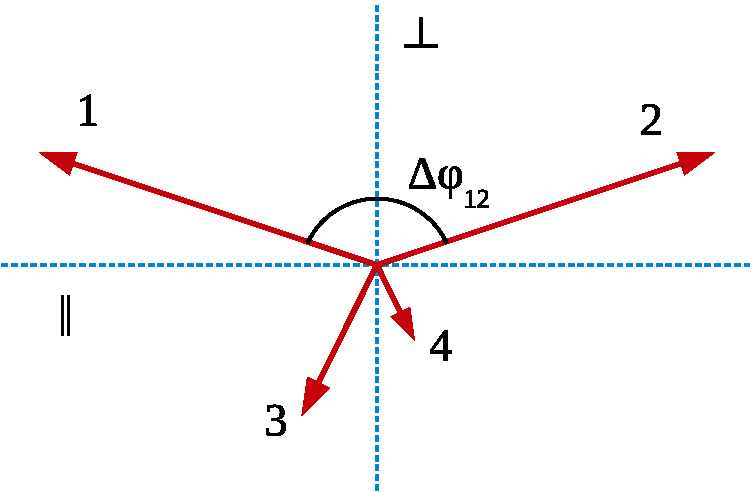
\includegraphics[width=0.45\textwidth]{figures/Sketch_Projections}
    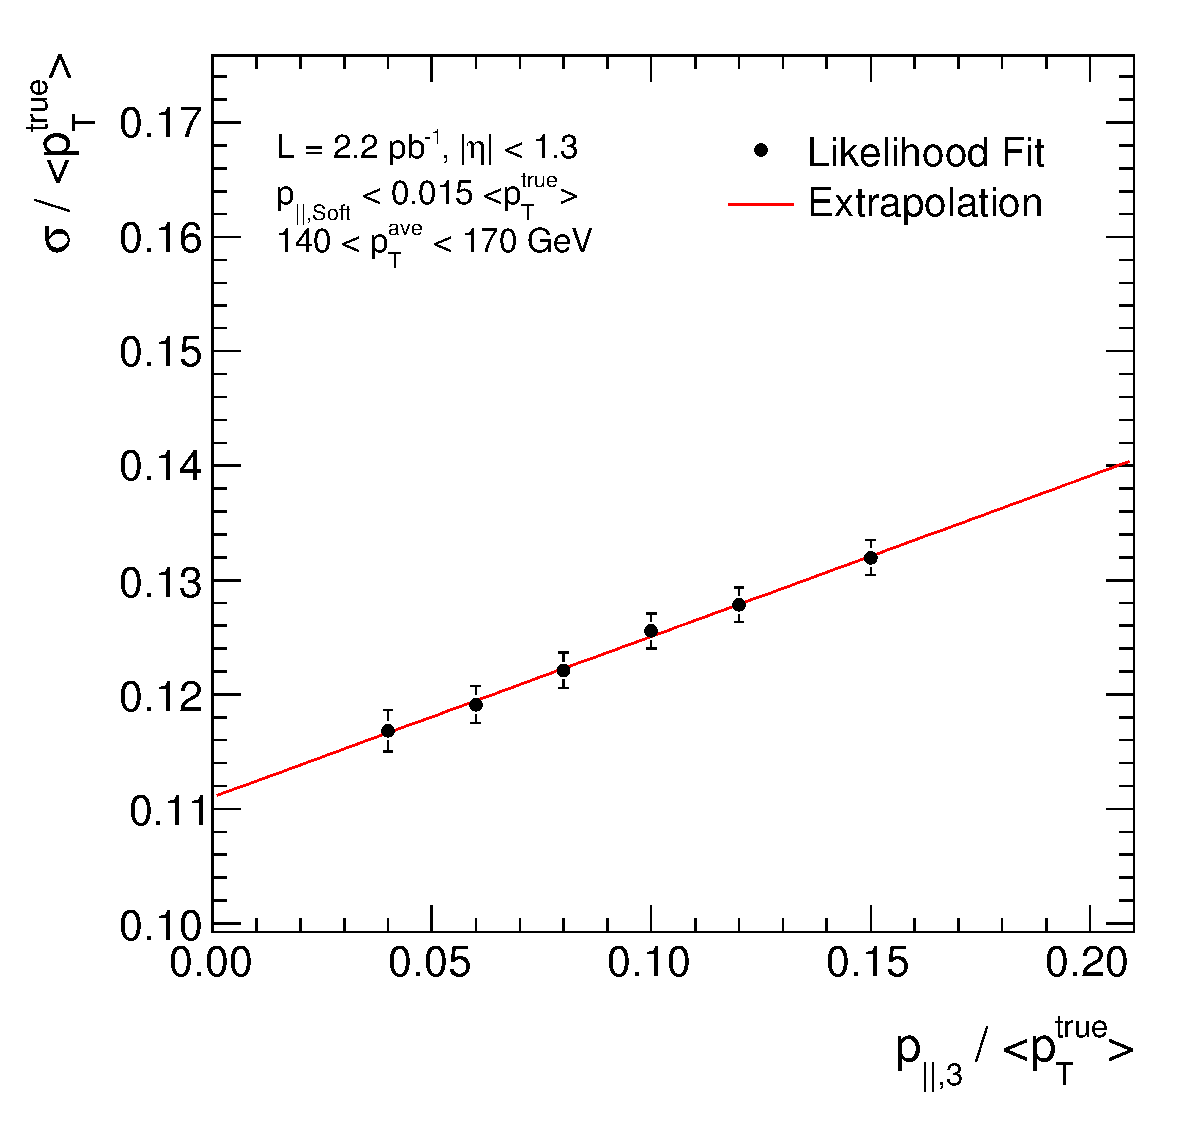
\includegraphics[width=0.45\textwidth]{figures/MaxLike_Data132440-144011_Eta00-13_ExtrapolatedPar0_PtBin4}\\
  \end{tabular}
  \caption{(\textit{Left}) Definition of the dijet axis $\phi_{||}$, the direction normal to the
    angle bisector of the leading two jets in the transverse plane.
    Additional jets with \pt components along $\phi_{||}$ will cause
    a \pt imbalance of the particle jets and bias the measured
    resolution towards larger values.
    (\textit{Right}) Gaussian resolutions \mbox{$\sigma/\mean{\pttrue}$} measured with the unbinned
    fit in Collider data for \mbox{$140 < \ptave < 170\gev$} and different \ppi{3}
    thresholds after suppression of additional soft jet activity along
    $\phi_{||}$. 
    \mbox{$\sigma/\mean{\pttrue}$} on \ppi{3} is linearly
    extrapolated to the case of an ideal dijet event.
  }
  \label{fig:qcd:resolMaxlike:biasAddJets}
\end{figure}


Fluctuations in the hadronisation processes lead to constituents which
are not clustered to the jet (\textit{out-of-cone}) and hence affect the measured response.
This bias is corrected using the MC simulation as it is small, of the
order of $1\%$:
The width of the \ptgen asymmetry, $\sigma(A^{\text{gen}})$ is determined for the
 case of perfectly balanced dijet events, using the
same extrapolation technique as above.
The measured jet \pt resolution is corrected for out-of-cone effects
by subtracting $\sqrt{2}\cdot\sigma(A^{\text{gen}})$ in quadrature.



\textit{From original draft}

As discussed in the previous Section~\ref{sec:ResFit:QCDMC:AddJetAct},
the presence of additional jets in the dijet event biases the
measurement towards larger resolutions and thus has to be corrected
for.
The size of the particle level jet \pt imbalance is correlated with the
measured relative \pt of the third jet as illustrated in Fig.~\ref{}.
Hence, in order to compensate for the bias in a data driven manner, different dijet samples with different thresholds of \ptrel (comp. step~1 of the event selection, Section~\ref{sec:ResFit:QCDMC:EvtSel}) are selected and the maximum likelihood fit is performed each time.
Then, the resulting resolution is extrapolated to the case of a two jet only event i.e. \mbox{$\ptrel\rightarrow0$}.

The approach chosen in the following is to define sufficiently small bins of jet \pt and measure the w.r.t. \pt average response in each bin for different limits \mbox{$\ptrel<x$}.
This is motivated by the fact that in case of a Gaussian response parametrisation (Section~\ref{sec:ResFit:QCDMC:Gauss}) there is then only one parameter $\bar{\sigma}$, which can be extrapolated relatively straight forward.
The chosen \pt and $\eta$ binning is listed in Table~\ref{tab:ResFit:QCDMC:Extrapolation:Binning}.
\begin{table}[ht]
  \caption{Definition of \pt bins for the fit of the mean Gaussian resolution.}
  \centering
  \begin{tabular}{cl|ccccccccc}
    \toprule
    \multicolumn{2}{c}{$|\eta|$ bin} & \multicolumn{9}{c}{\pt bin edges $(\text{Ge}\kern-0.06667em\text{V})$} \\
    \midrule
    \multirow{2}{*}{$0$} & \multirow{2}{*}{$(0 - 1.2)$} & 80 & 100 & 120 & 140 & 170 & 200 & 250 & 300 & 350 \\
    && 400 & 500 & 600 & 800 & 1000 \\
    $1$ & $(1.2 - 2.6)$ & 60 & 80 & 100 & 120 & 150 & 200 & 300 &  500 & 700 \\
    $2$ & $(2.6 - 3.2)$ & 80 & 100 & 150 &&&&&&\\
    \bottomrule
  \end{tabular}
  \label{tab:ResFit:QCDMC:Extrapolation:Binning}
\end{table}

Was the Gaussian parametrised with a \pt dependent $\sigma$ as e.g. in~\eqref{eq:ResFit:ToyMC:Sigma}, the correlation of the parameter $\xi_{i}$ of $\sigma$ would have to be taken into account in contrast.
Note that this is exactly the case for the Crystal Ball response parametrisation (Section~\ref{sec:ResFit:QCDMC:CrystalBall}), and additional work is foreseen to de-correlate the parameters $\sigma$, $\alpha$, and $n$.

In the following, the particle level differential dijet cross section is taken from the interpolated \ptgen distribution Fig.~\ref{fig:ResFit:QCDMC:Extrapolation:Gauss:ExBin:SpectrumAndExtrapolation} (\textit{left}) that has been obtained from the Monte Carlo truth information. 



\subsubsection{Measurement of the Gaussian response function}\label{sec:ResFit:QCDMC:Gauss}

A sample of dijet events is selected for each $\eta$, \pt bin listed in Table~\ref{tab:ResFit:QCDMC:Extrapolation:Binning}.
The selection bias (Section~\ref{sec:ResFit:Method:Biases}) is incorporated in the probability density function as before, comp. Fig.~\ref{fig:ResFit:QCDMC:Extrapolation:Gauss:ExBin:SpectrumAndExtrapolation} (\textit{left}).

\begin{figure}[ht]
  \centering
  \begin{tabular}{cc}
    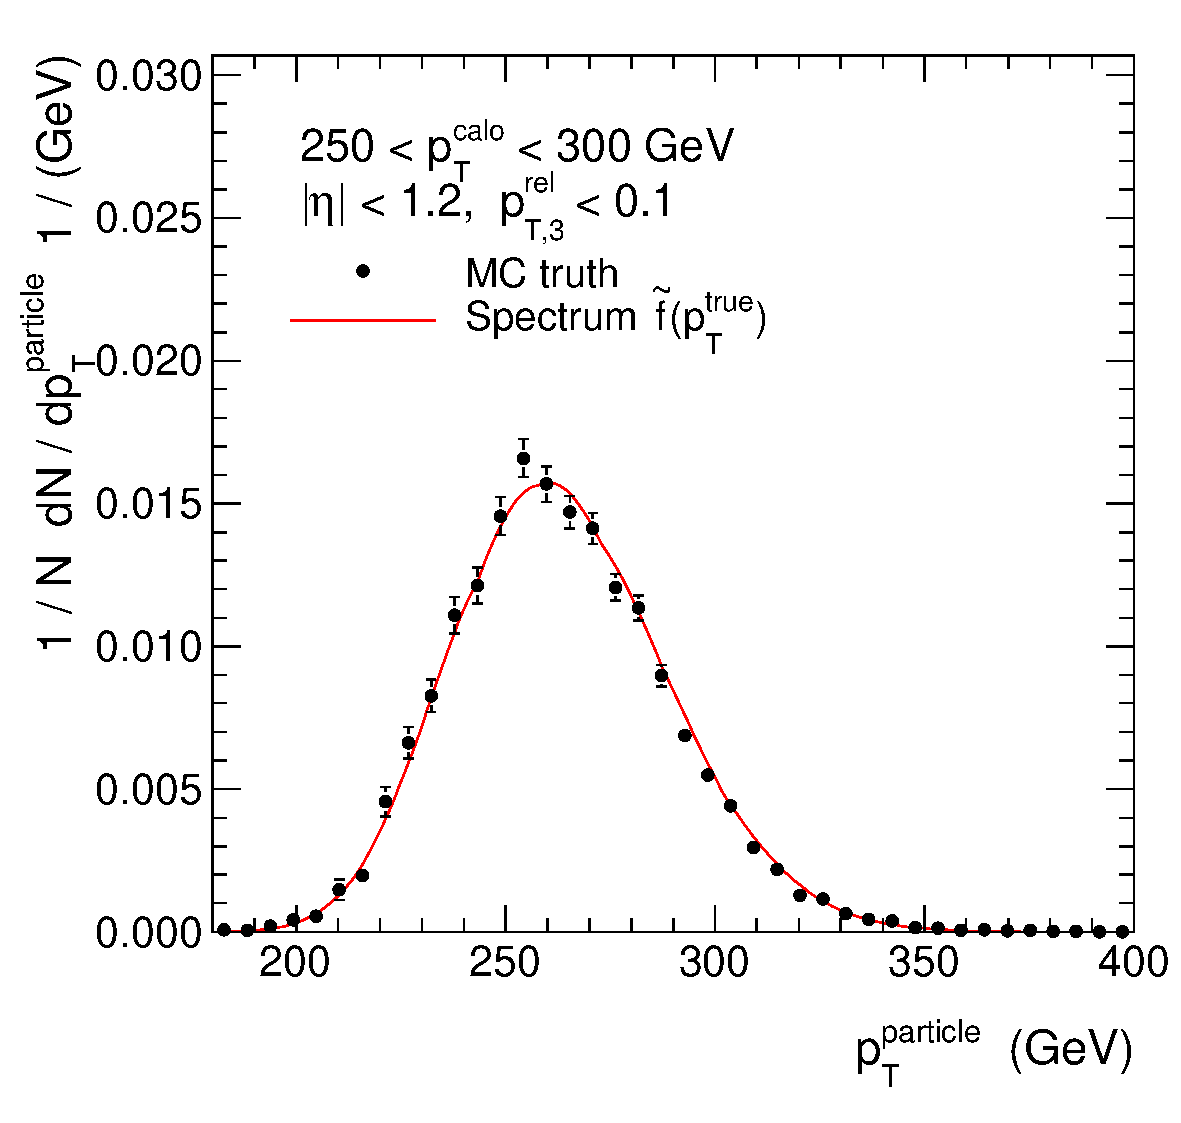
\includegraphics[width=0.45\textwidth]{figures/ResFit_Spring10QCDFlat_Gauss_Eta0_Spectrum_PtBin6} &
    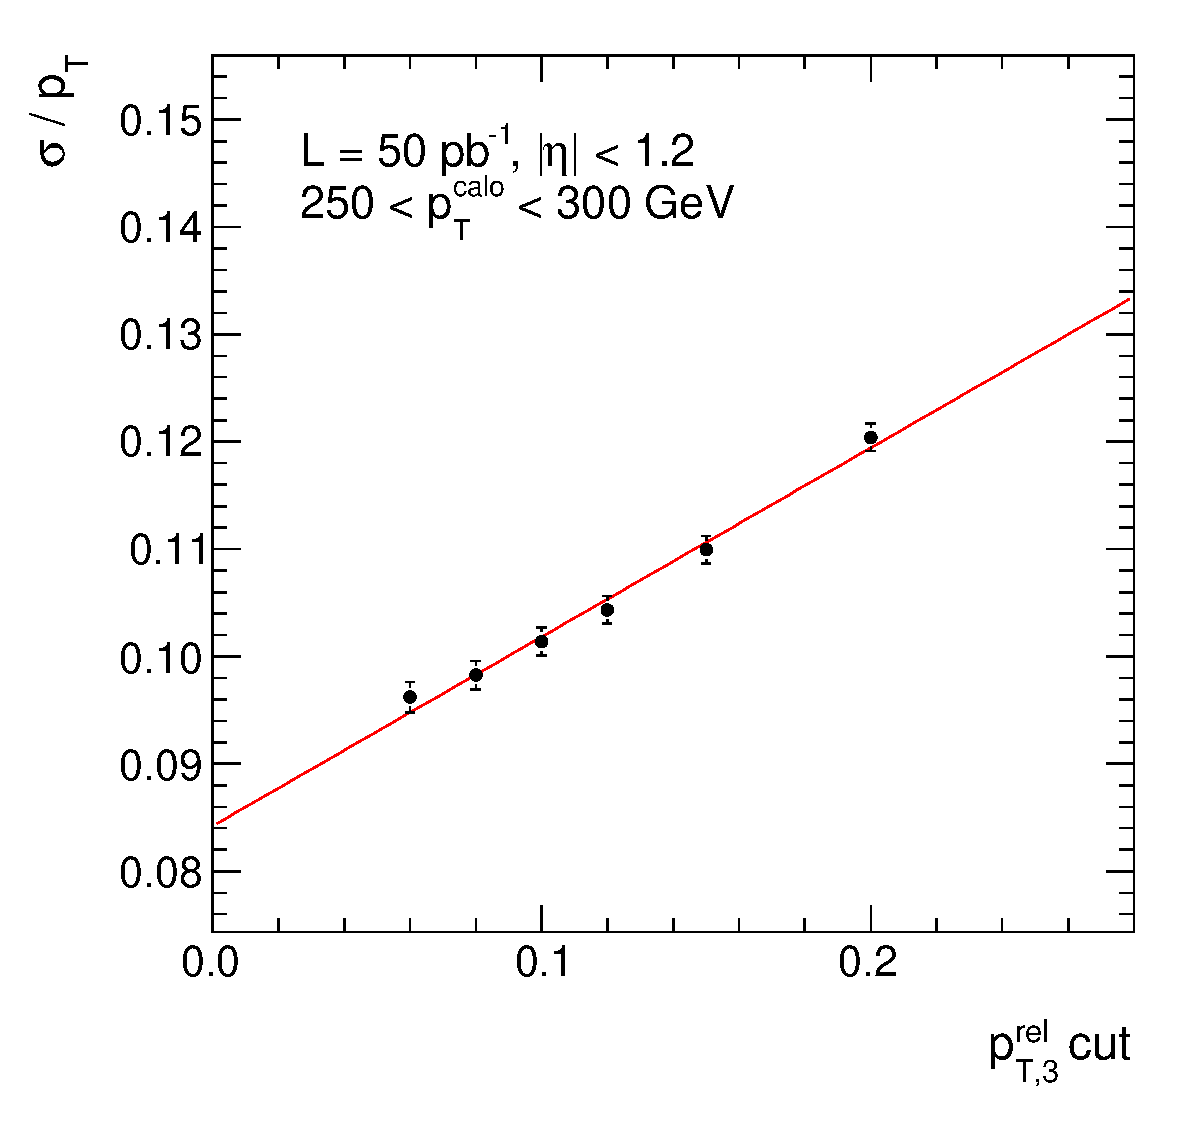
\includegraphics[width=0.45\textwidth]{figures/ResFit_Spring10QCDFlat_Gauss_Eta0_ExtrapolatedPar0_PtBin6}
  \end{tabular}
\caption{(\textit{Left}) The parametrisation of the realistic particle jet \pt spectrum in one \pt bin as used in the dijet likelihood (solid line) in comparison to the prediction from Monte Carlo truth (full circles). 
  (\textit{Right}) $\bar{\sigma}/\pt$ from Gaussian fits for different maximal \ptrel in the same \pt bin.
  The solid line is a linear fit to extrapolate $\bar{\sigma}/\pt$ to the ideal case of only two jets in the
  final state.}
\label{fig:ResFit:QCDMC:Extrapolation:Gauss:ExBin:SpectrumAndExtrapolation}
\end{figure}

The mean Gaussian response
\begin{equation*}
  r_{\bar{\sigma}}\left(\pt|\pttrue\right) = 
  \frac{1}{\sqrt{2\pi}\bar{\sigma}}\exp\left[-\frac{1}{2}\left(\frac{\pt - \pttrue}{\bar{\sigma}}\right)^{2}\right]
\end{equation*}
is measured in each bin by maximising the likelihood~\eqref{eq:ResFit:Likelihood} w.r.t.~$\bar{\sigma}$.
The fitted relative Gaussian widths $\bar{\sigma}/\pt$ in one \pt bin are shown in Fig.~\ref{fig:ResFit:QCDMC:Extrapolation:Gauss:ExBin:SpectrumAndExtrapolation} (\textit{right}) for different thresholds on \ptrel.
Here, \pt is the mean value of the assumed spectrum~$\tilde{f}(\pttrue)$ in that bin, shown Fig.~\ref{fig:ResFit:QCDMC:Extrapolation:Gauss:ExBin:SpectrumAndExtrapolation} (\textit{left}).
In order to extrapolate the measurements to the case of a two jet only event, the $\bar{\sigma}/\pt$ are fitted with a linear function --- shown as a solid line --- and the $y$ axis intercept is taken as the corrected jet \pt resolution.

The jet \pt spectra, fitted Gaussian resolutions $\bar{\sigma}/\pt$ versus \ptrel, and the extrapolation are shown in Appendix~\ref{sec:ResFit:App:AllResults:Gauss} for all \pt and $\eta$ bins.

\begin{figure}[ht]
  \centering
  \begin{tabular}{cc}
    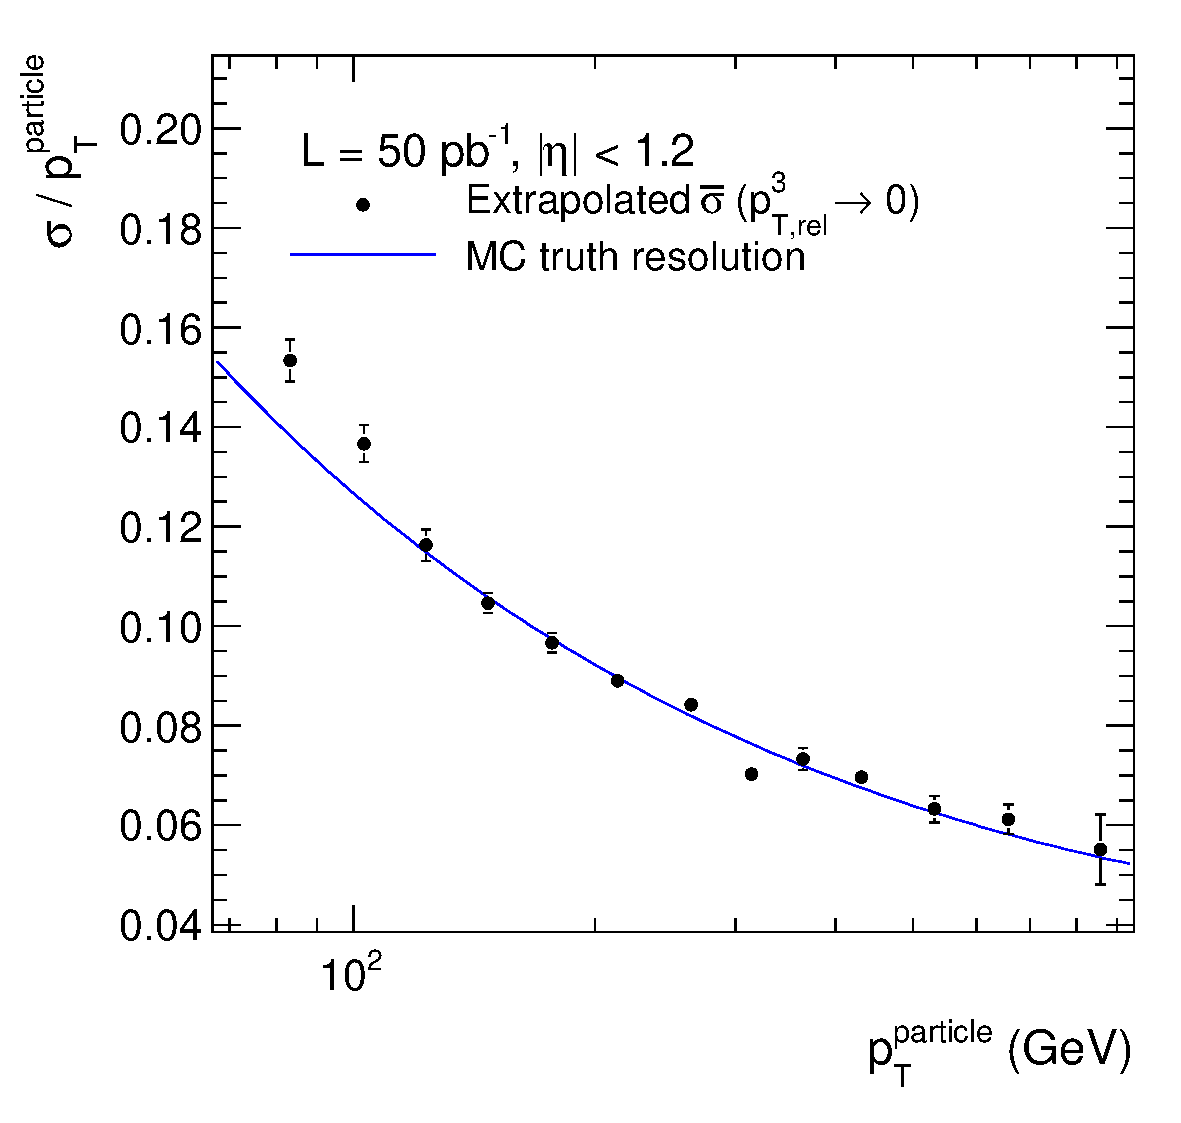
\includegraphics[width=0.45\textwidth]{figures/ResFit_Spring10QCDFlat_Gauss_Eta0_ExtrapolatedResolution} &
    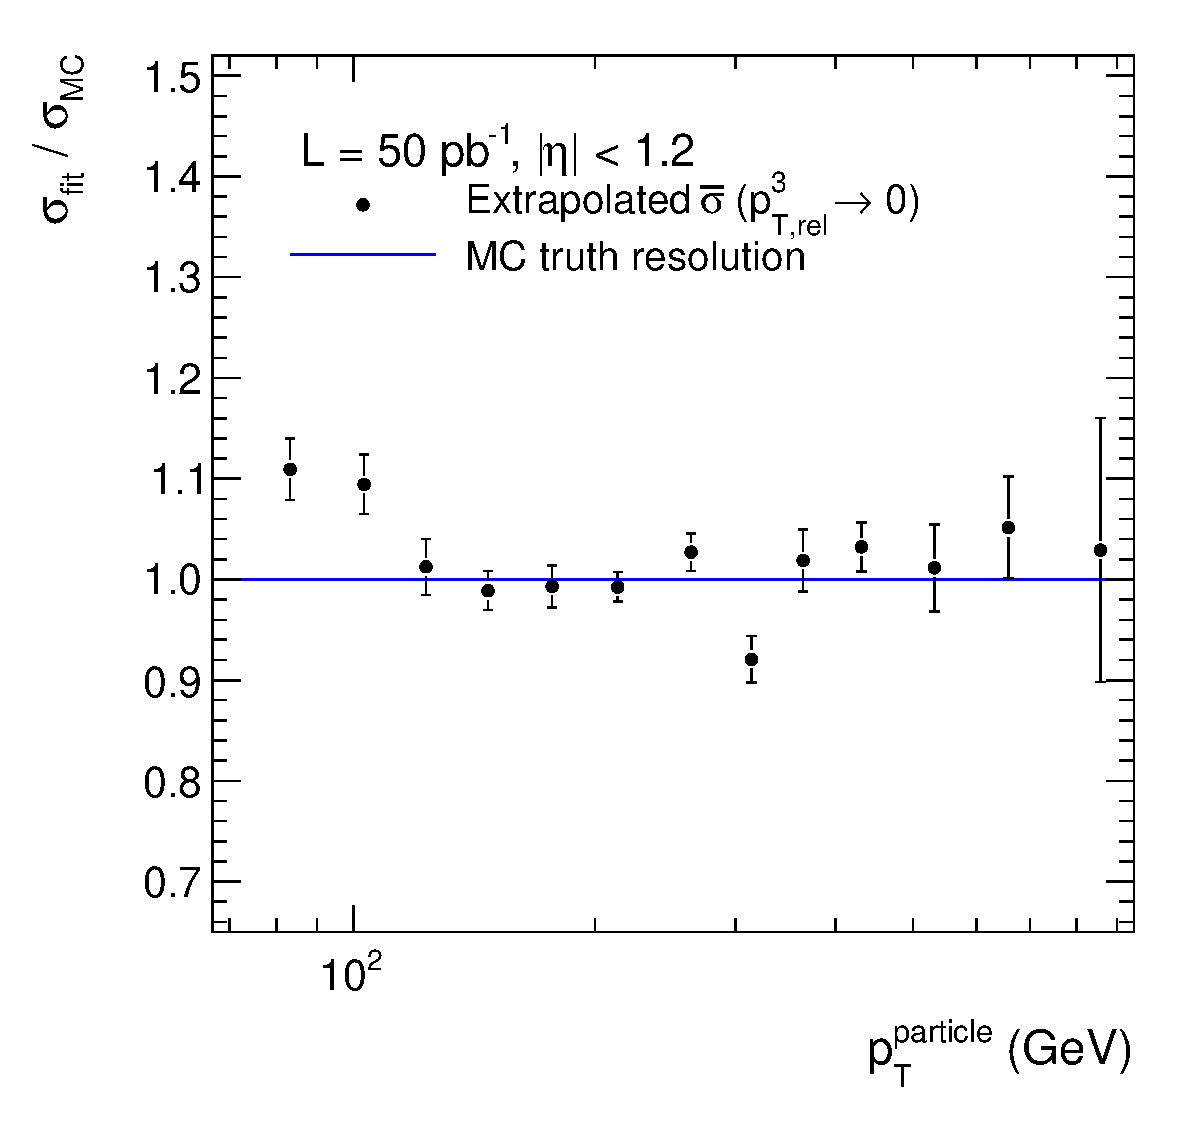
\includegraphics[width=0.45\textwidth]{figures/ResFit_Spring10QCDFlat_Gauss_Eta0_ExtrapolatedResolutionRatio}
  \end{tabular}
\caption{(\textit{Left}) Fitted Gaussian jet \pt resolutions, $\bar{\sigma}/\pt$, from extrapolations for \mbox{$\ptrel\rightarrow0$} in different \pt bins.
  The \pt are the mean values of $\tilde{f}(\pttrue)$ in each bin.
  The error bars indicate the combined statistical uncertainties from the extrapolation and the Monte Carlo statistics.
  The dashed line shows the Monte Carlo truth resolution for comparison.
  (\textit{Right}) Ratio of fitted and Monte Carlo truth resolution.}
\label{fig:ResFit:QCDMC:Extrapolation:Gauss:ResoVsPt}
\end{figure}

The jet \pt resolution $\bar{\sigma}/\pt$ measurements, corrected for the effect of additional jet activity, are shown for different \pt bins in Fig.~\ref{fig:ResFit:QCDMC:Extrapolation:Gauss:ResoVsPt}.
(Again, the \pt are the mean values of the assumed spectrum~$\tilde{f}(\pttrue)$ in each bin.)
The fitted values are in good agreement with the Monte Carlo truth prediction, shown as a dash line.
The larger deviation in the two low \pt bins is assumed to be caused by the increasing influence of incorrect jet ordering due to the greater resolution on the extrapolation procedure\footnote{This effect is seen when using the dijet asymmetry method to measure jet \pt resolutions~\cite{bib:cmspas:dijetasymm}.}.

The error bars shown in Fig.~\ref{fig:ResFit:QCDMC:Extrapolation:Gauss:ResoVsPt} represent the combined statistical uncertainties of the fit and due to the Monte Carlo sample size:
\begin{enumerate}
\item The first contribution is the statistical uncertainty on the parameter of $y$ axis intercept in the linear extrapolation (Fig.~\ref{fig:ResFit:QCDMC:Extrapolation:Gauss:ExBin:SpectrumAndExtrapolation} (\textit{left})).
\item The second contribution arises from the uncertainty due to the limited Monte Carlo sample size.
 As the event weights are large for small \pt, statistical fluctuations become significant.
 In order to roughly evaluate this uncertainty, the same fits have been performed again without event weights (for the used sample this corresponds to a flattened QCD spectrum).
 The statistical uncertainties obtained in this case on the $y$ axis intercept are added in quadrature to the ones in 1.
 This procedure has to be improved to obtain a statistically correct description of the uncertainty.
\end{enumerate}

Due to the selection requirement \mbox{$\ptrel < x$}, all events selected for a particular value of $x$ in Fig.~\ref{fig:ResFit:QCDMC:Extrapolation:Gauss:ExBin:SpectrumAndExtrapolation} (\textit{right}) are also included in the samples selected with larger values of $x$.
Hence, the measured widths $\bar{\sigma}/\pt$ in one \pt are strongly correlated.
This correlation is not considered in the quoted uncertainties.
The planned treatment is to either include the correlations explicitly or perform the measurements in exclusive bins of \ptrel.
